
% -------------------
% Topology Management
% -------------------

A major challenge towards decentralized resource monitoring and control, is to federate all devices (that we also refer to as peers following the peer-to-peer literature) in an abstraction layer (an overlay network) that allows intercommunication and efficient resource discovery. Given that this is a classic Peer to Peer (P2P) problem, this section provides context about P2P systems and the taxonomy of overlay networks.

In P2P, participants (peers) contribute to the system with a portion of their resources, so that the overall system can accomplish tasks which would otherwise be impossible for a single peer to solve. Typically, this is achieved in a decentralized way, which means peers must establish neighboring connections among themselves to enable information exchange which, in turn, enables to progress towards the system goals. 

Participants in a P2P system may know all other peers in the system, which is typically referred to as \textbf{full membership} knowledge, this is a popular approach in Cloud systems. However, as the system scales to larger numbers of peers, concurrently entering and leaving the system (a phenomenon called churn \cite{stutzbach2006understanding}), this information becomes costly to maintain up-to-date. 

In order to circumvent the aforementioned problems, a common alternative is to have peers only maintain a view of a subset of all peers in the system, which is called \textbf{partial membership}. This information is maintained by some membership algorithm which restricts neighboring relations among peers. Partial membership solutions are attractive because they offer similar functionality to full membership systems, while achieving more scalability and resiliency to churn. Neighboring relations may be unidirectional or bidirectional, and the combination of these relations is what materializes an \textbf{overlay network}.

\subsection{Taxonomy of Overlay Networks}

Overlay networks are logical networks which operate at the applicational level, these rely on an existing network (commonly referred to as the \textit{underlay}) to establish neighboring relations, where each participant tipically only communicates directly with its overlay neighbors \cite{leitaoPHDthesis}. Overlays are commonly designed towards specific applicational needs, as such, their neighboring relations may or may not follow some sort of logic. As observable in Figure \ref{fig:overlay_networks}, there are two main categories of overlays: \textbf{structured} and \textbf{unstructured}:

\subsubsection*{Unstructured Overlays}

Unstructured overlays usually impose little to no rules in neighboring relations, peers may pick random peers to be their neighbors, or alternatively employ strategies to "rank"\ neighbors and selectively pick the "best" given a particular criteria that is typically entwined with the needs of applications. A key factor of unstructured overlays is their low maintenance cost, given that nodes can easily create neighboring relations and replace failed ones, consequently, this is the type of overlay which offers better resilience to churn.

\begin{figure}
    \centering
    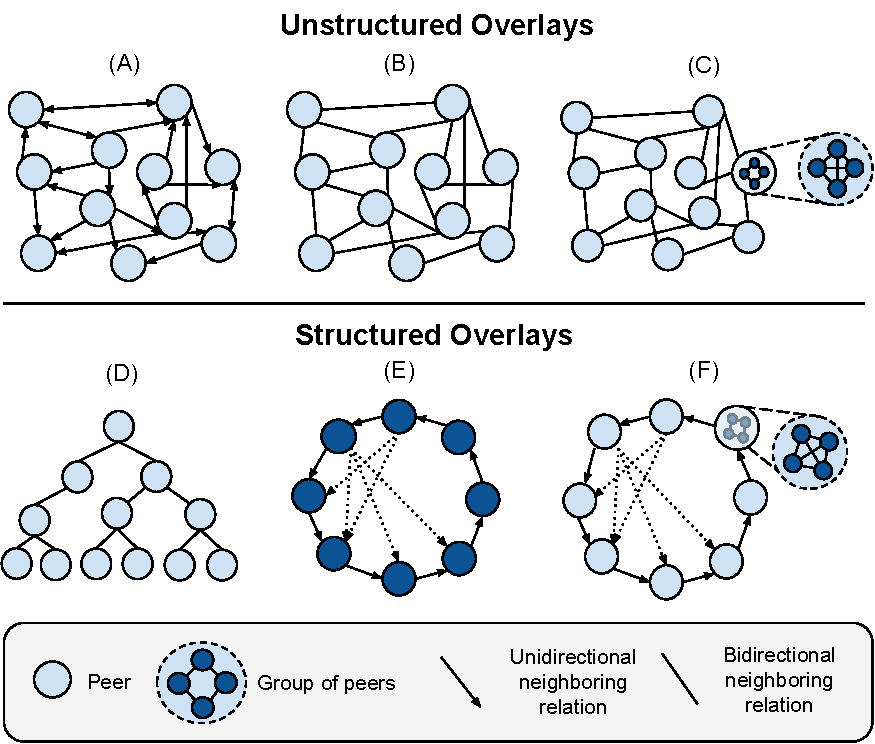
\includegraphics[width=0.60\linewidth]{Figures/overlay_networks.pdf}
    \caption{Examples Overlay Networks}
    \label{fig:overlay_networks}
\end{figure}


In figure \ref{fig:overlay_networks} we ilustrate three examples of unstructured overlay networks: (A) is a representation of an overlay network where the connections are unidirectional (e.g. Cyclon \cite{jelasity2007gossip}), in this type of overlay peers have no control over the status of incoming connections, consequently, a peer may become isolated from the network without realizing it, which is undesirable. 

Overlay (B) is similar to (A), however, neighboring connections are bidirectional. This means that a peer with a given number of outgoing connections must also have the correspondent number of incoming connections, diminishing the risk of the peer becoming disconnected from the overlay (this is the approach taken by HyParView \cite{Hyparview} to achieve high reliability and fault-tolerance).

Lastly, (C) is a representation of an unstructured overlay where peers establish groups among themselves (such as Overnesia \cite{leitao2014overnesia}). Grouping multiple devices into a group can be useful because: (1) failures can be quickly identified and resolved by other members of the group; (2) nodes can replicate data within the group, leading to increased availability of that data; (3) for devices with low computing capabilities groups are useful because nodes have nearby neighbors which can simplify the offload of computational tasks. 

\subsubsection*{Structured Overlays}

Structured overlays enforce stronger rules towards neighbor selection (generally based on identifiers of peers). As a result, the overlay generally converges to a a certain topology known a priori (e.g., a circle, tree, hypercube, among others). 

In Figure \ref{fig:overlay_networks} illustrate three kinds of structured overlay networks: (D) corresponds to a tree, trees are widely used to perform broadcasts (e.g., PlumTree \cite{leitao2007epidemic}) because of the smaller message complexity required to deliver a message to all nodes, or to monitor the system state (if nodes in lower levels of the tree periodically send monitoring information to upper levels in the tree, in turn, the root of the node has a global view of the collected monitoring information (e.g., Astrolabe \cite{Renesse2003})). However, trees are very fragile in the presence of faults \cite{leitao2007epidemic}.

Overlay depicted in (E) corresponds to the overlay topology tipically expected to support Distributed Hash Tables. These overlays are extremely popular due to their effective applicational-level routing capabilities. In a DHT, peers employ a global coordination mechanism which restricts their neighboring relations such that can find any peer \textit{responsible} for any given key in a small limited number of steps.

In the example that we show in (E), the topology consists of a ring (which is the strategy employed by Chord \cite{stoica2003chord}), however, not all distributed hash tables rely on rings to perform effective routing. For example, in Kademlia \cite{maymounkov2002kademlia}, nodes organized across a leave in a binary tree.

Finally, the overlay denoted in (C) is similar to overlay (E), however, each position of the DHT consists of a virtual node composed by multiple physical nodes (which is the strategy employed by Rollerchain \cite{rollerchain}). Because of this, routing procedures have the potential to be load-balanced, and churn effects are mitigated, because the failure of a physical node does necessarily mean the failure of a virtual node. 
 
\subsection{Overlay Network Metrics}

If we look at an overlay network where connections between nodes represent edges and nodes represent vertices in a graph, we obtain a graph from which we may extract direct metrics to estimate overlay performance \cite{leitaoPHDthesis}:

\begin{enumerate}
    
    \item \textbf{Connectivity}. This property is usually measured as a percentage, corresponding to the largest portion of the system that is connected, intuitively, a connected graph is one where there is at least one path from each node to all other nodes in the system.
    
    \item \textbf{Degree Distribution}. The degree of a node consists in the number of arcs that are connected to it. In a directed graph, there is a distinction between \textbf{in-degree} and \textbf{out-degree} of a node,nodes with a high in-degree value have higher reachability, while nodes with 0 in-degree cannot be reached. The out-degree of a node represents a measure of the contribution of that node towards the maintenance of the overlay topology.
    
    \item \textbf{Average Shortest Path}. A path is composed by the edges of the graph that a message would have to cross to get from one node to other. The average shortest path consists in the average of all shorter paths between every pair of peers. To promote efficient communication patterns, is desirable that this value is as low as possible.
    
    \item \textbf{Clustering Coefficient}. The clustering coefficient provides a measure of the density of neighboring relations across the neighbors of links between a given node. It consists in the number of a node's neighbors divided by the maximum number of links that could exist between those neighbors. A high value of clustering coefficient means that there is a higher amount of redundant communication among nodes.
    
    \item \textbf{Overlay Cost}. If we assume that a link in the overlay has a \textit{cost}, (e.g. derived from latency) then the overlay cost is the sum of all the costs of the links that form the overlay. 
    
\end{enumerate}

\subsection{Examples of Overlay Networks}

\textbf{T-MAN} \cite{jelasity2005t} is protocol to manage the topology of overlay networks based on a gossiping scheme, which proposes to build a wide range of structured overlay networks (e.g., ring, mesh, tree, etc.). To achieve this, T-MAN takes an overlay as an input to the protocol, this overlay is then organized by taking into consideration a ranking method applied by every node to compare the preference among possible neighbors iteratively. 

Nodes periodically exchange their neighboring sets with peers in the system and keep the nodes which rank higher according to the ranking method. A limitation of T-Man is that it does not ensure stability of the in-degree of nodes during the optimization of the overlay, and consequently, the overlay may not remain connected. 

\textbf{Management Overlay Network} \cite{liang2005mon} (MON) is an overlay network system aimed at facilitating the management of large distributed applications.
MON builds on-demand overlay structures that allow users to execute instant management commands, such as query the current status of the application, or push software updates to all the nodes. This means that MON does not have a cost when there are no commands running.

The on-demand overlay construction allows the creation of two Overlay Networks: trees and direct acyclic graphs. These overlays, in turn, can be employed towards aggregating monitoring data related to the status of the devices. Limitations from using MON are that the resulting overlays are susceptible to topology mismatch, and do not ensure connectivity. Furthermore, since the topologies are supposed to be short-lived, MON does not provide mechanisms for dealing with faults.

\textbf{Hyparview} \cite{Hyparview} (Hybrid Partial View) gets its name from maintaining two exclusive views: the \textit{active} and \textit{passive} view, which are distinguished by their maintenance strategy. 

The \textit{passive view} is a larger view which consists of a random set of peers in the system, this view is maintained by a simple gossip protocol which periodically gossips a message to a random peer in the active view. This message contains a subset of the neighbors of the sending node and a time-to-live (TTL), the message is forwarded in the system until the TTL expires. In contrast, the \textit{active view} is a smaller view (around log(n)) created during the bootstrap of the protocol, and actively maintained by monitoring peers with a TCP connection (effectively making the active view connections bidirectional and act as a failure detector). Whenever peers from the active view fail (detected by the active TCP conntection), nodes attempt to replace them with nodes in the passive view.

Hyparview is often used as a \textit{peer sampling service} for other protocols which rely on the connections from the active view to collaborate (e.g. PlumTree \cite{leitao2007epidemic}). It achieves high reliability even in the face of high percentage of node failures, however, the resulting topology is flat, which is not desirable given the taxonomy of edge environments we are considering. Furthermore, it may suffer from topology mismatch, because of the random nature of neighboring connections, the resulting topology may mismatch the underlying network.

\textbf{X-BOT} \cite{leitao2012x} is a protocol which constructs an unstructured overlay network where neighboring relations are biased  considering a particular, and parametrizable, metric. This metric is provided by an \textit{oracle}, the oracle is a component that exports a function which accepts a pair of peers and attributes a cost to that neighboring connection. An oracle may take into account device latency, ISP distribution, network stretch, among others. 

The rationale X-BOT is as follows: nodes maintain active and passive views similar to Hyparview \cite{Hyparview}. Then, nodes periodically trigger optimization rounds where they attempt to bias a portion of their connections according to the oracle. This potentually addresses the previous concerns about the overlay topology mismatching the underlying network, however, it still proposes a flat topology, which also is not adequate for the edge environment taxonomy. 

\textbf{Overnesia} \cite{leitao2014overnesia} is a protocol which establishes an overlay composed of fully connected groups of nodes, where all nodes within a group share the same identifier. Nodes join the system by sending a JOIN request to a bootstrap node which triggers a random walk, the requesting node joins the group where its random walk terminates (either because it finds an underpopulated group or because the TTL expires). 

Intra-group membership consistency is enforced by an anti-entropy mechanism where nodes within a group periodically exchange messages containing their own view of the group. When a group detects that its size has become too large, it triggers a dividing procedure where splits the groups in two halves. Conversely, when the group size has fallen bellow a certain threshold, nodes trigger a collapse procedure, where each node takes the initiative to relocate itself to another group, resulting in the graceful collapse of the group. Finally, inter-group links are acquired by propagating random walks throughout the overlay.

As previously mentioned, establishing groups of nodes enables load-balancing, efficient dissemination of queries, and fault-tolerance. However, limitations from Overnesia arise from peers maintaining active connections to all members belonging to the same group, and keeping the group membership up-to-date, which may limit system scalability, finally, the overlay may suffer from topology mismatch, as two nodes within the same group may be distant in the underlay.

\textbf{Chord} \cite{stoica2003chord} is a well known structured overlay network where the protocol builds and manages a ring topology, similar to overlay (E) in Figure \ref{fig:overlay_networks}. Each node is assigned an m-bit identifier that is uniformly distributed in the id space. Then, peers are ordered by identifier in a clockwise circle, where any data piece identified by \(k\), is assigned to the first peer whose identifier is equal or follows k in the identifier space. 

Chord implements a system of "shortcuts"\ called the \textbf{finger table}. The finger table contains at most \(m\) entries, each $ith$ entry of this table corresponds to the first peer that succeeds a certain peer \(n\) by \(2^{ith}\) in the circle. This means that whenever the finger table is up-to-date, and the system is stable, lookups for any data piece only take logarithmic time to finish. 

Although Chord provides the best trade-off between bandwidth and lookup latency \cite{dht_performance_churn}, it has its limitations: peers do not learn routing information from incoming requests, links have no correlation to latency or traffic locality, and the overlay is highly susceptible to churn. Finally, the ring topology is flat, which means that lower capacity nodes in the ring may become a limitation instead of an asset in the context of routing procedures.

%Chord is the building block for many other solutions: Cyclone \cite{Artigas2005} is a hierarchical DHT inspired on Chord which constructs clusters by splitting the ID space into a PREFIX and SUFIX. The PREFIX provides intra-cluster identity, whereas the SUFIX lets nodes know their residence cluster.

%Hieras \cite{1240580} uses a binning scheme according the underlay topology to group peers into smaller rings. The lower the ring, the smaller the average link latency. Routing is done in lower rings to make use of the reduced latency and if the resource is not present in those rings, then the query is forwarded to higher rings.

%Crescendo \cite{Ganesan2004} splits the ID range into domains (similar to DNS), where nodes in leaf-domains form Chord rings, then nodes merge rings by applying rules such that rings in different domains can communicate. The resulting routing table and the routing procedures in Crescendo are similar to Chord.


\textbf{Pastry} \cite{rowstron2001pastry} is another well known DHT which assigns a 128-bit node identifier (nodeId) to each peer in the system. The nodes are randomly generated, and consequently, are uniformly distributed in the 128-bit nodeId space. 

The routing procedure is as follows: in each routing step, messages are forwarded to nodes whose nodeId shares a prefix that is at least one bit closer to the key, if there are no nodes available, Pastry routes messages towards the numerically closest nodeId. This routing procedure takes O(log N) routing steps, where N is the number of Pastry nodes in the system. This protocol has been widely used and acts as a building block for Pub-Sub applications such as Scribe \cite{10.1007/3-540-45546-9_3} and file storage systems like PAST \cite{990064}. 

Limitations from using Pastry arise from the use of a numeric distance function towards the end of the routing process, which creates discontinuities at some node ID values, and complicates attempts at formal analysis of worst case behavior, in addition to the flat topology which mismatches the edge device taxonomy.

\textbf{Tapestry} \cite{tapestry} Is a DHT similar to pastry, however, nodeIDs are represented taking into account a certain base b supplied as a parameter of the system. Routing procedures in the overlay are similar to pastry, messages are incrementally forwarded to the destination digit by digit (e.g. ***8 -> **98 -> *598 -> 4598), consequently, routing procedures theoretically take logb(n) hops to their destination where b is the base of the ID space. Because nodes assume that the preceding digits all match the current node's suffix, nodes in Tapestry only need to keep a constant size of entries at each route level, consequently, nodes contain entries for a fixed-sized neighbor map of size b.log(N).  

\textbf{Kademlia} \cite{maymounkov2002kademlia} is a DHT where nodes are considered leaves in a binary tree. Kademlia nodes are assigned 160-bit identifiers uniformly distributed in the identifiers space. Peers route queries and locate data pieces by employing an \textbf{XOR-based distance function} which is symmetric and unidirectional. Each node in Kademlia is a router where its routing tables consist of shortcuts to peers whose XOR distance is between \(2^{i}\) by \(2^{i + 1}\) in the ID space, given the use of the XOR metric, "closer"\ nodes are those that share a longer common prefix.

The main benefits that Kademlia draws from this approach are: nodes learn routing information from receiving messages, there is a single routing algorithm for the whole routing process (unlike Pastry \cite{rowstron2001pastry}) which eases formal analysis of worst-case behavior. Finally, Kademlia exploits the fact that node failures are inversely related to uptime by prioritizing nodes that are already present in the routing table.

\textbf{Kelips} \cite{gupta2003kelips} is a group-based DHT which exploits increased memory usage and constant background communication to achieve reduced lookup time and message complexity. Kelips nodes are split in $k$ affinity groups split in the intervals [0,$k-1$] of the identifier space, thus, with $n$ nodes in the system, each affinity group contains $\frac{n}{k}$ peers. Within a group, nodes store a partial set of nodes contained in the same affinity group and a small set of nodes lying in foreign affinity groups. With this architecture, Kelips achieves O(1) time and message complexity in lookups, however, it has limited scalability when compared to previous DHTs, given the increased memory consumption (O($\sqrt{n}$).

\textbf{Rollerchain} \cite{rollerchain} is a protocol which establishes a group-based DHT by leveraging on techniques from both structured and unstructured  overlays (Chord and Overnesia). In short, the Overnesia protocol materializes an unstructured overlay composed by logical groups of physical peers who share the same identifier. Then, the peer with the lowest identifier within each logical group joins a structured overlay, obtains the adresses of other virtual peers, and distributes them among group members.

Rollerchain has the potential to enable a type of replication which has higher robustness to churn events when compared to other other replication strategies, however, there are limitations to this approach: (1) the load is unbalanced within members of each group, as only one node  is in charge of populating and balancing the inter-group links; (2) similar to Chord, nodes do not learn from incoming queries, which contrasts with other DHTs such as Pastry; (3) the protocol has a higher maintenance cost when compared to a regular DHT.

\subsection{Discussion}

Unstructured overlays are an attractive option towards federating large amounts of devices in heavily dynamic environments. They provide a low clustering coefficient, are flexible, and maintain good connectivity even in the face of churn. However, given their unstructured nature, they are limited in certain scenarios, for example, when trying to find a specific peer in the system.

Conversely, distributed hash tables enable efficient routing procedures with very low message overhead, which makes them suitable for application-level routing. However, given their strict neighboring rules, participating nodes cannot replace neighbors easily, which hinders the fault-tolerance of these types of topologies, in addition, given the fact that devices in edge environments have varied computational power and connectivity, they may become a limitation instead of an asset in the context of routing procedures. 

%Hierarchical DHTS consisting of DHTS contained within other DHTS (e.g. a ring within a ring) offer several advantages over a flat DHT: first, lookups take less hops and messages to reach the target, second, organizing nodes in disjoint groups allows traffic locality if groups of nodes are close within the underlay, and churn events within a group stay contained within that group. 

%However, many of these systems either employ more memory to accommodate the many levels of the hierarchy, or tradeoff reliability (by shortening the number of connections) for memory and communication efficiency. 

